\newpage

\subsection{Prototipo a escala}

\noindent
\justify

Se han desarrollado estudios experimentales sobre un prototipo a escala de una planta de extracci\'on con capacidad productiva de $1 [kg / bache]$, tres baches al d\'ia. El flujo de trabajo se puede apreciar en la Figura \ref{cadena}.

\begin{figure}[h!]
	\centering
	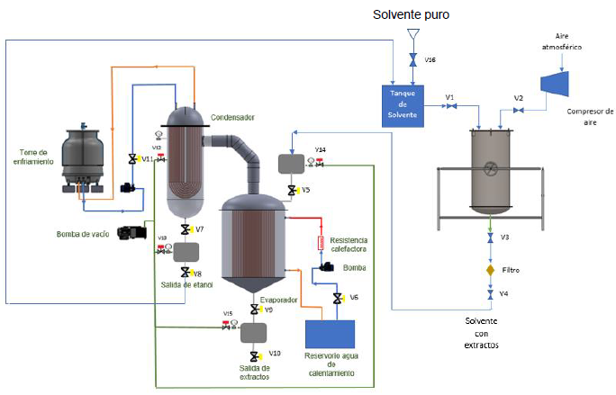
\includegraphics[width=1.1\textwidth]{Images/planta.PNG}
	\caption{Prototipo desarrollado$^{\cite{Proyecto, Patente2018}}$.}
	\label{cadena}
\end{figure}

La invenci\'on desarrollada consiste de:
\begin{itemize}
	\item Molino de bolas dise\~nado como recipiente a presi\'on.
	\item Unidad compresora de aire.
	\item Evaporador.
	\item Condensador.
	\item Sistema de calentamiento de agua por resistencia el\'ectrica.
	\item Torre de enfriamiento.
\end{itemize}


